%\right) %\documentclass[conference]{IEEEtran}
%\documentclass[10pt, conference, letterpaper]{IEEEtran}
\documentclass[conference]{IEEEtran}


\usepackage{amsfonts}
\usepackage{amssymb}
\usepackage{amsmath}
\usepackage{algorithm}
\usepackage[noend]{algorithmic}
\usepackage{color}
\usepackage{graphicx}
\usepackage{subfigure}
\usepackage{comment}
\usepackage[strings]{underscore}
\usepackage{comment}
\usepackage{url}



\hyphenation{op-tical net-works semi-conduc-tor}
\setlength{\parskip}{0.1em}
\renewcommand{\baselinestretch}{1}

\begin{document}


\title{DSP Matlab Assignment \\Designing Low Pass Filters with MATLAB}
\author{\IEEEauthorblockN{Vincent Martin}
\IEEEauthorblockA{
Department of Electrical Engineering\\
Temple University, Philadelphia, PA, USA \\
Email: \{vince.p.martin\}@temple.edu }
}

\maketitle

%\vspace*{-0.5cm}
\begin{abstract}


\end{abstract}
This report reviews how MATLAB can be used to construct a low pass filter. The construction of such a filter is used on a noisy .wav audio file to determine what its contents are. MATLAB code is included.

\section{Introduction}
Filters are used to alter data that are passed through it based on the frequency of that data. For example, a low pass filter would be used to pass only values that are determined to be under the set cutoff frequency that the designer has determined. Additionally there are other filters such as high pass filters that pass only data that is above the cutoff frequency and finally, band pass filters that are a combination of both low and high pass filters. This report will walk through the construction of a low pass filter by using one to filter a noisy .wav file.

\section{Construction of the Low Pass Filter}
Constructing the low pass filter in MATLAB requires that we determine values for the pass band frequency (Fpass), stop band frequency (Fstop), pass band ripple (Apass) and the stop band attenuation (Astop). Figure \ref{figure:filter} displays all of these values visually.

\begin{figure}[H]
\centering
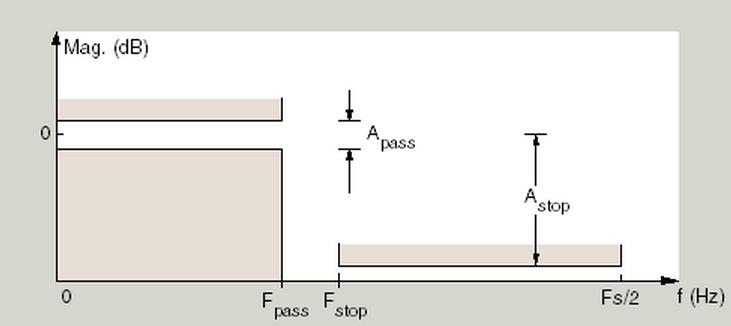
\includegraphics[width=3.0in]{./figures/filter.png}
\caption{Low Pass Filter.}
\label{figure:filter}
\end{figure}

\subsection{Preparing the Data}
Before constructing the filter it is important that the .wav file is imported into the matlab environment.

Additionally it is also important to note that the function used to build filters in MATLAB does not take Hz as an input. Due to this Hz must be altered into a normalized value. This is done in the code via a function called freqNormlized that will be included along with this report.

\subsection{Determining the Pass Band Frequency}
The pass band value determines which frequencies are allowed to pass through the filter. In order to determine which value would be appropriate a MATLAB program was written that would iterate through frequency values from 100Hz to 3000Hz at 100Hz intervals. Once this was done a low pass filter was constructed for each value and the sound was played. 

\subsection{Determining the Stop Band Frequency}
Once a proper value for the pass band was determined the next step was is to experiment with different stop band frequencies. A similar approach was taken by iterating through proper values, with this time starting at the the value that was above the chosen pass band frequency. Each filter was experimented with and then played. 

\subsection{Determining the Pass Band Ripple}
Once proper values were found for the pass band and the stop band the same code was used to try a few different values for the pass band. The values that were attempted were 0.01,0.0001,0.1,1,10,20,30 and 40.

\subsection{Determining the Stop Band Attenuation}
The last value that had to be determined was the stop band attenuation. This was again done via the same code loop and the values cycled through were 10,20,30,40,50,60 and 100.

\section{Results}
\subsection{Wav File Analysis}
The sound file says "Flights from Denver to San Francisco."

Table \ref{table:filterValues} displays the values that were chosen for the filter.

\begin{table}[h]
\begin{tabular}{|l|l|l|l|l|}
\hline
\textbf{Filter}            & \textbf{Fpass} & \textbf{Fstop} & \textbf{Apass (Db)} & \textbf{Astop (Db)} \\ \hline
Chosen via Experimentation & 0.3               & 0.325               &  0.0001              & 100               \\ \hline
Chosen via Analysis        & 0.35               & 0.36               &   0.0001             & 100               \\ \hline
\end{tabular}
\label{table:filterValues}
\caption{Values for Filter}
\end{table}

Figure \ref{figure:beforeFilter} displays the magnitude of the sound file before the filter was applied. Figure \ref{figure:afterFilter} displays the magnitude of the sound file after the filter has been applied.

\begin{figure}[H]
\centering
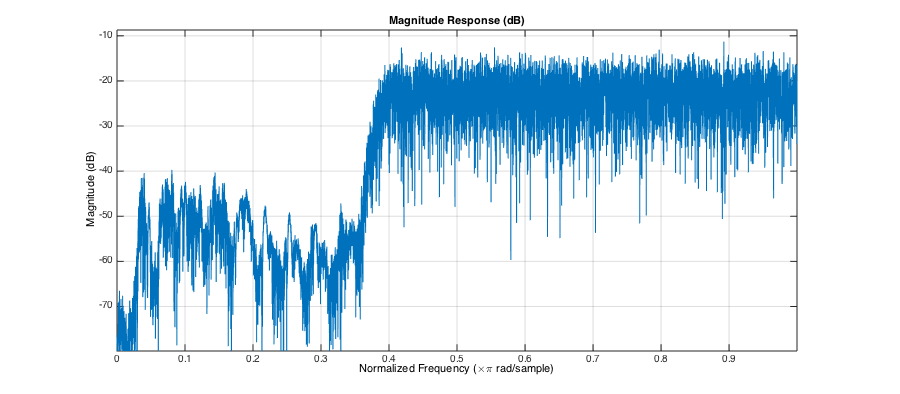
\includegraphics[width=3.0in]{./figures/before_filter.png}
\caption{Before Filter.}
\label{figure:beforeFilter}
\end{figure}

\begin{figure}[H]
\centering
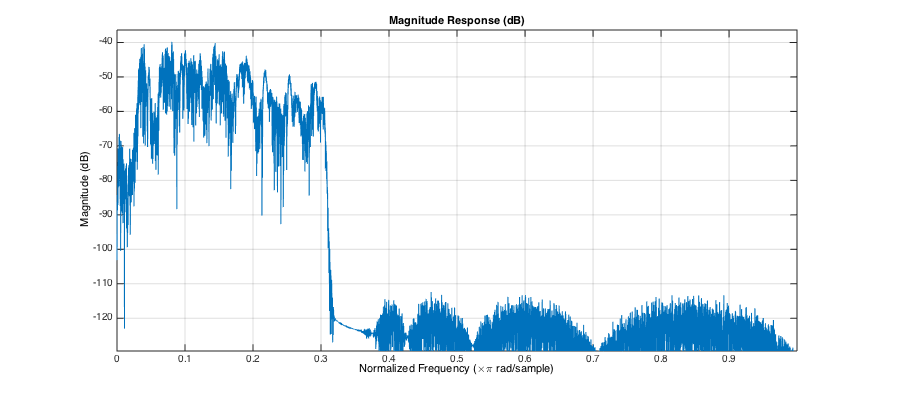
\includegraphics[width=3.0in]{./figures/after_filter.png}
\caption{After Filter.}
\label{figure:afterFilter}
\end{figure}

\section{Conclusion}
Noise was able to be scrubbed from the sound file. This is quite helpful as the sound file was completely useless before this. It is interesting to note that altering the Fstop value did not show much change to the file. However, changing the Apass to a larger value caused the file to echo. Also, using a smaller value for the Astop caused the file to be quite noisy. Settling with a value of 100Db for the Astop was the final step that made the file end up being quite clear.

{\footnotesize
\bibliographystyle{IEEEtran}
\bibliography{glass-video}
}
\end{document}


